\documentclass[svgnames,11pt]{beamer}
\input{/home/tof/Documents/Cozy/latex-include/preambule_commun.tex}
\input{/home/tof/Documents/Cozy/latex-include/preambule_beamer.tex}
%\usepackage{pgfpages} \setbeameroption{show notes on second screen=left}
\author[]{Christophe Viroulaud}
\title{Exercices arbres\\Correction}
\date{\framebox{\textbf{Algo 05}}}
%\logo{}
\institute{Terminale - NSI}

\begin{document}
\begin{frame}
\titlepage
\end{frame}
\section{Exercice 1}
\begin{frame}
    \frametitle{Exercice 1}

    \begin{itemize}
\item racine: A
\item 9 feuilles
\item taille: 16
\item profondeur: 3
\end{itemize}

\end{frame}
\begin{frame}
    \frametitle{}
    \begin{center}
        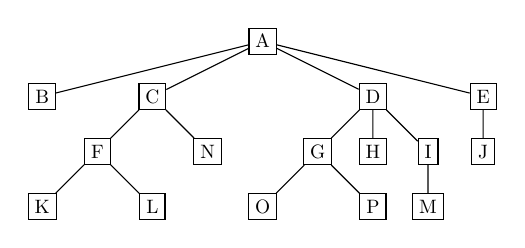
\begin{tikzpicture}[scale=0.7, transform shape]
            \node[draw] (A) at (0,0) {A};
            \node[draw] (B) at (-4,-1) {B};
            \node[draw] (C) at (-2,-1) {C};
            \node[draw] (D) at (2,-1) {D};
            \node[draw] (E) at (4,-1) {E};
            \node[draw] (F) at (-3,-2) {F};
            \node[draw] (N) at (-1,-2) {N};
            \node[draw] (G) at (1,-2) {G};
            \node[draw] (H) at (2,-2) {H};
            \node[draw] (I) at (3,-2) {I};
            \node[draw] (J) at (4,-2) {J};
            \node[draw] (K) at (-4,-3) {K};
            \node[draw] (L) at (-2,-3) {L};
            \node[draw] (M) at (3,-3) {M};
            \node[draw] (O) at (0,-3) {O};
            \node[draw] (P) at (2,-3) {P};

            \draw (A) -- (B);
            \draw (A) -- (C);
            \draw (A) -- (D);
            \draw (A) -- (E);
            \draw (C) -- (F);
            \draw (C) -- (N);
            \draw (D) -- (G);
            \draw (D) -- (H);
            \draw (D) -- (I);
            \draw (E) -- (J);
            \draw (F) -- (K);
            \draw (F) -- (L);
            \draw (G) -- (O);
            \draw (G) -- (P);
            \draw (I) -- (M);
        \end{tikzpicture}
    \end{center}
    \begin{itemize}
        \item parcours en largeur: A B C D E F N G H I J K L O P M
        \item parcours en profondeur:
        \begin{itemize}
            \item préfixe: A B C F K L N D G O P H I M E J
            \item infixe: B A K F L C N O G P D H M I J E
            \item suffixe: B K L F N C O P G H M I D J E A
        \end{itemize}
    \end{itemize}

\end{frame}
\section{Exercice 2}
\begin{frame}
    \frametitle{Exercice 2}
    \begin{itemize}
        \item Windows: taille = 22; hauteur = 2
        \item Linux: taille = 35; hauteur = 3
        \end{itemize}
    

\end{frame}
\section{Exercice 3}
\begin{frame}[fragile]
    \frametitle{Exercice 3}

    \begin{center}
    \begin{lstlisting}[language=Python , basicstyle=\ttfamily\small, xleftmargin=2em, xrightmargin=2em]
dictionnaire = ['arbre', 'arbres', 'arbitre', 'arbitrent', 'arbitrer', 'arbitres', 'arbitrez', 'arbitrons', 'binaire', 'binaires', 'binette', 'binettes', 'bio', 'empile', 'empilent' 'empiler', 'empiles', 'empilez', 'empilons', 'exact', 'exacte', 'exactes', 'exacts']
\end{lstlisting}
    \captionof{code}{\centering 23 éléments dans la liste et 22 tests pour trouver \emph{exactes}.}
    \label{CODE}
    \end{center}

\end{frame}
\begin{frame}
    \frametitle{}

    \begin{center}
        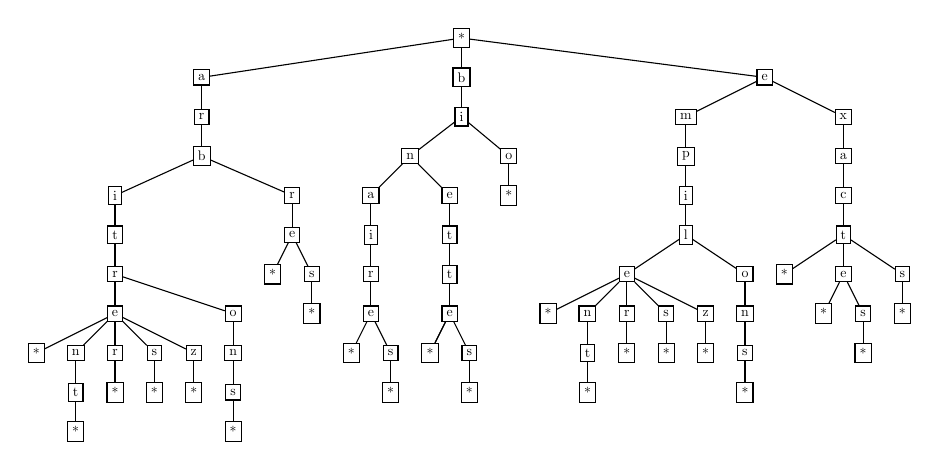
\begin{tikzpicture}[scale=0.5, transform shape]
        \node[draw] (0) at (-11,0) {*};
        \node[draw] (1) at (-7,0) {*};
        \node[draw] (3) at (-11,1) {t};
        \node[draw] (4) at (-10,1) {*};
        \node[draw] (5) at (-9,1) {*};
        \node[draw] (6) at (-8,1) {*};
        \node[draw] (7) at (-7,1) {s};
        \node[draw] (8) at (-3,1) {*};
        \node[draw] (9) at (-1,1) {*};
        \node[draw] (10) at (2,1) {*};
        \node[draw] (11) at (6,1) {*};
        \node[draw] (12) at (-12,2) {*};
        \node[draw] (13) at (-11,2) {n};
        \node[draw] (14) at (-10,2) {r};
        \node[draw] (15) at (-9,2) {s};
        \node[draw] (16) at (-8,2) {z};
        \node[draw] (17) at (-7,2) {n};
        \node[draw] (18) at (-4,2) {*};
        \node[draw] (19) at (-3,2) {s};
        \node[draw] (20) at (-2,2) {*};
        \node[draw] (21) at (-1,2) {s};
        \node[draw] (22) at (2,2) {t};
        \node[draw] (23) at (3,2) {*};
        \node[draw] (24) at (4,2) {*};
        \node[draw] (25) at (5,2) {*};
        \node[draw] (26) at (6,2) {s};
        \node[draw] (27) at (9,2) {*};
        \node[draw] (28) at (-10,3) {e};
        \node[draw] (29) at (-7,3) {o};
        \node[draw] (30) at (-5,3) {*};
        \node[draw] (31) at (-3.5,3) {e};
        \node[draw] (32) at (-1.5,3) {e};
        \node[draw] (33) at (1,3) {*};
        \node[draw] (34) at (2,3) {n};
        \node[draw] (35) at (3,3) {r};
        \node[draw] (36) at (4,3) {s};
        \node[draw] (37) at (5,3) {z};
        \node[draw] (38) at (6,3) {n};
        \node[draw] (39) at (8,3) {*};
        \node[draw] (40) at (9,3) {s};
        \node[draw] (41) at (10,3) {*};
        \node[draw] (42) at (-10,4) {r};
        \node[draw] (43) at (-6,4) {*};
        \node[draw] (44) at (-5,4) {s};
        \node[draw] (45) at (-3.5,4) {r};
        \node[draw] (46) at (-1.5,4) {t};
        \node[draw] (47) at (3,4) {e};
        \node[draw] (48) at (6,4) {o};
        \node[draw] (49) at (7,4) {*};
        \node[draw] (50) at (8.5,4) {e};
        \node[draw] (51) at (10,4) {s};
        \node[draw] (52) at (-10,5) {t};
        \node[draw] (53) at (-5.5,5) {e};
        \node[draw] (54) at (-3.5,5) {i};
        \node[draw] (55) at (-1.5,5) {t};
        \node[draw] (56) at (4.5,5) {l};
        \node[draw] (57) at (8.5,5) {t};
        \node[draw] (58) at (-10,6) {i};
        \node[draw] (59) at (-5.5,6) {r};
        \node[draw] (60) at (-3.5,6) {a};
        \node[draw] (61) at (-1.5,6) {e};
        \node[draw] (62) at (0,6) {*};
        \node[draw] (63) at (4.5,6) {i};
        \node[draw] (64) at (8.5,6) {c};
        \node[draw] (65) at (-7.8,7) {b};
        \node[draw] (66) at (-2.5,7) {n};
        \node[draw] (67) at (0,7) {o};
        \node[draw] (68) at (4.5,7) {p};
        \node[draw] (69) at (8.5,7) {a};
        \node[draw] (70) at (-7.8,8) {r};
        \node[draw] (71) at (-1.2,8) {i};
        \node[draw] (72) at (4.5,8) {m};
        \node[draw] (73) at (8.5,8) {x};
        \node[draw] (74) at (-7.8,9) {a};
        \node[draw] (75) at (-1.2,9) {b};
        \node[draw] (76) at (6.5,9) {e};
        \node[draw] (77) at (-1.2,10) {*};
        
        \draw (0) -- (3);
        \draw (1) -- (7);
        \draw (3) -- (13);
        \draw (4) -- (14);
        \draw (5) -- (15);
        \draw (6) -- (16);
        \draw (7) -- (17);
        \draw (8) -- (19);
        \draw (9) -- (21);
        \draw (10) -- (22);
        \draw (11) -- (26);
        \draw (12) -- (28);
        \draw (13) -- (28);
        \draw (14) -- (28);
        \draw (15) -- (28);
        \draw (16) -- (28);
        \draw (17) -- (29);
        \draw (18) -- (31);
        \draw (19) -- (31);
        \draw (20) -- (32);
        \draw (20) -- (32);
        \draw (21) -- (32);
        \draw (22) -- (34);
        \draw (23) -- (35);
        \draw (24) -- (36);
        \draw (25) -- (37);
        \draw (26) -- (38);
        \draw (27) -- (40);
        \draw (28) -- (42);
        \draw (30) -- (44);
        \draw (31) -- (45);
        \draw (32) -- (46);
        \draw (33) -- (47);
        \draw (34) -- (47);
        \draw (35) -- (47);
        \draw (36) -- (47);
        \draw (37) -- (47);
        \draw (38) -- (48);
        \draw (39) -- (50);
        \draw (40) -- (50);
        \draw (41) -- (51);
        \draw (42) -- (29);
        \draw (42) -- (52);
        \draw (43) -- (53);
        \draw (44) -- (53);
        \draw (45) -- (54);
        \draw (46) -- (55);
        \draw (47) -- (56);
        \draw (48) -- (56);
        \draw (49) -- (57);
        \draw (50) -- (57);
        \draw (51) -- (57);
        \draw (52) -- (58);
        \draw (53) -- (59);
        \draw (54) -- (60);
        \draw (55) -- (61);
        \draw (56) -- (63);
        \draw (57) -- (64);
        \draw (58) -- (65);
        \draw (59) -- (65);
        \draw (60) -- (66);
        \draw (61) -- (66);
        \draw (62) -- (67);
        \draw (63) -- (68);
        \draw (64) -- (69);
        \draw (65) -- (70);
        \draw (66) -- (71);
        \draw (67) -- (71);
        \draw (68) -- (72);
        \draw (69) -- (73);
        \draw (70) -- (74);
        \draw (71) -- (75);
        \draw (72) -- (76);
        \draw (73) -- (76);
        \draw (74) -- (77);
        \draw (75) -- (77);
        \draw (76) -- (77);
        
        \end{tikzpicture}
        \captionof{figure}{\centering 8 tests pour trouver \emph{exactes}.}
        \label{dico}
        \end{center}

\end{frame}
\end{document}